\documentclass[10pt,journal,compsoc]{IEEEtran}
\usepackage{xspace}
\usepackage{caption}

\usepackage[dvipsnames]{xcolor}
\usepackage[bookmarks=false]{hyperref}

\newcommand\myshade{85}
\colorlet{mylinkcolor}{violet}
\colorlet{mycitecolor}{YellowOrange}
\colorlet{myurlcolor}{Aquamarine}
\hypersetup{
  linkcolor  = mylinkcolor!\myshade!black,
  citecolor  = mycitecolor!\myshade!black,
  urlcolor   = myurlcolor!\myshade!black,
  colorlinks = true,
}

\usepackage{graphicx}

\graphicspath{{gfx/},{plots/}}
\DeclareGraphicsExtensions{.pdf,.jpeg,.png}
\providecommand{\norm}[1]{\lVert#1\rVert}

% *** CITATION PACKAGES ***
%
\ifCLASSOPTIONcompsoc
  \usepackage[nocompress]{cite}
\else
  % normal IEEE
  \usepackage{cite}
\fi


\usepackage[cmex10]{amsmath}
\usepackage{amsfonts}
\usepackage{multirow}
\usepackage{rotating}
\usepackage{booktabs}




% *** SPECIALIZED LIST PACKAGES ***
%
\usepackage{algorithm}
\usepackage{algorithmic}
\usepackage{array}
\usepackage{mdwmath}
\usepackage{mdwtab}
\usepackage{calc}
\usepackage{epstopdf}



% Also highly recommended is Mark Wooding's extremely powerful MDW tools,
% especially mdwmath.sty and mdwtab.sty which are used to format equations
% and tables, respectively. The MDWtools set is already installed on most
% LaTeX systems. The lastest version and documentation is available at:
% http://www.ctan.org/tex-archive/macros/latex/contrib/mdwtools/


% IEEEtran contains the IEEEeqnarray family of commands that can be used to
% generate multiline equations as well as matrices, tables, etc., of high
% quality.


%\usepackage{eqparbox}
% Also of notable interest is Scott Pakin's eqparbox package for creating
% (automatically sized) equal width boxes - aka "natural width parboxes".
% Available at:
% http://www.ctan.org/tex-archive/macros/latex/contrib/eqparbox/

% *** SUBFIGURE PACKAGES ***
% \ifCLASSOPTIONcompsoc
% \usepackage[tight,normalsize,sf,SF]{subfigure}
% \else
% \usepackage[tight,footnotesize]{subfigure}
% \fi
% subfigure.sty was written by Steven Douglas Cochran. This package makes it
% easy to put subfigures in your figures. e.g., "Figure 1a and 1b". For IEEE
% work, it is a good idea to load it with the tight package option to reduce
% the amount of white space around the subfigures. Computer Society papers
% use a larger font and \sffamily font for their captions, hence the
% additional options needed under compsoc mode. subfigure.sty is already
% installed on most LaTeX systems. The latest version and documentation can
% be obtained at:
% http://www.ctan.org/tex-archive/obsolete/macros/latex/contrib/subfigure/
% subfigure.sty has been superceeded by subfig.sty.


% \ifCLASSOPTIONcompsoc
%  \usepackage[caption=false]{caption}
%  \usepackage[font=normalsize,labelfont=sf,textfont=sf]{subfig}
% \else
%  \usepackage[caption=false]{caption}
%  \usepackage[font=footnotesize]{subfig}
% \fi
% subfig.sty, also written by Steven Douglas Cochran, is the modern
% replacement for subfigure.sty. However, subfig.sty requires and
% automatically loads Axel Sommerfeldt's caption.sty which will override
% IEEEtran.cls handling of captions and this will result in nonIEEE style
% figure/table captions. To prevent this problem, be sure and preload
% caption.sty with its "caption=false" package option. This is will preserve
% IEEEtran.cls handing of captions. Version 1.3 (2005/06/28) and later 
% (recommended due to many improvements over 1.2) of subfig.sty supports
% the caption=false option directly:
\ifCLASSOPTIONcompsoc
 \usepackage[caption=false,font=normalsize,labelfont=sf,textfont=sf]{subfig}
\else
 \usepackage[caption=false,font=footnotesize]{subfig}
\fi


% The latest version and documentation can be obtained at:
% http://www.ctan.org/tex-archive/macros/latex/contrib/subfig/
% The latest version and documentation of caption.sty can be obtained at:
% http://www.ctan.org/tex-archive/macros/latex/contrib/caption/




% *** FLOAT PACKAGES ***
%
%\usepackage{fixltx2e}
% fixltx2e, the successor to the earlier fix2col.sty, was written by
% Frank Mittelbach and David Carlisle. This package corrects a few problems
% in the LaTeX2e kernel, the most notable of which is that in current
% LaTeX2e releases, the ordering of single and double column floats is not
% guaranteed to be preserved. Thus, an unpatched LaTeX2e can allow a
% single column figure to be placed prior to an earlier double column
% figure. The latest version and documentation can be found at:
% http://www.ctan.org/tex-archive/macros/latex/base/



%\usepackage{stfloats}
% stfloats.sty was written by Sigitas Tolusis. This package gives LaTeX2e
% the ability to do double column floats at the bottom of the page as well
% as the top. (e.g., "\begin{figure*}[!b]" is not normally possible in
% LaTeX2e). It also provides a command:
%\fnbelowfloat
% to enable the placement of footnotes below bottom floats (the standard
% LaTeX2e kernel puts them above bottom floats). This is an invasive package
% which rewrites many portions of the LaTeX2e float routines. It may not work
% with other packages that modify the LaTeX2e float routines. The latest
% version and documentation can be obtained at:
% http://www.ctan.org/tex-archive/macros/latex/contrib/sttools/
% Documentation is contained in the stfloats.sty comments as well as in the
% presfull.pdf file. Do not use the stfloats baselinefloat ability as IEEE
% does not allow \baselineskip to stretch. Authors submitting work to the
% IEEE should note that IEEE rarely uses double column equations and
% that authors should try to avoid such use. Do not be tempted to use the
% cuted.sty or midfloat.sty packages (also by Sigitas Tolusis) as IEEE does
% not format its papers in such ways.




%\ifCLASSOPTIONcaptionsoff
%  \usepackage[nomarkers]{endfloat}
% \let\MYoriglatexcaption\caption
% \renewcommand{\caption}[2][\relax]{\MYoriglatexcaption[#2]{#2}}
%\fi
% endfloat.sty was written by James Darrell McCauley and Jeff Goldberg.
% This package may be useful when used in conjunction with IEEEtran.cls'
% captionsoff option. Some IEEE journals/societies require that submissions
% have lists of figures/tables at the end of the paper and that
% figures/tables without any captions are placed on a page by themselves at
% the end of the document. If needed, the draftcls IEEEtran class option or
% \CLASSINPUTbaselinestretch interface can be used to increase the line
% spacing as well. Be sure and use the nomarkers option of endfloat to
% prevent endfloat from "marking" where the figures would have been placed
% in the text. The two hack lines of code above are a slight modification of
% that suggested by in the endfloat docs (section 8.3.1) to ensure that
% the full captions always appear in the list of figures/tables - even if
% the user used the short optional argument of \caption[]{}.
% IEEE papers do not typically make use of \caption[]'s optional argument,
% so this should not be an issue. A similar trick can be used to disable
% captions of packages such as subfig.sty that lack options to turn off
% the subcaptions:
% For subfig.sty:
% \let\MYorigsubfloat\subfloat
% \renewcommand{\subfloat}[2][\relax]{\MYorigsubfloat[]{#2}}
% For subfigure.sty:
% \let\MYorigsubfigure\subfigure
% \renewcommand{\subfigure}[2][\relax]{\MYorigsubfigure[]{#2}}
% However, the above trick will not work if both optional arguments of
% the \subfloat/subfig command are used. Furthermore, there needs to be a
% description of each subfigure *somewhere* and endfloat does not add
% subfigure captions to its list of figures. Thus, the best approach is to
% avoid the use of subfigure captions (many IEEE journals avoid them anyway)
% and instead reference/explain all the subfigures within the main caption.
% The latest version of endfloat.sty and its documentation can obtained at:
% http://www.ctan.org/tex-archive/macros/latex/contrib/endfloat/
%
% The IEEEtran \ifCLASSOPTIONcaptionsoff conditional can also be used
% later in the document, say, to conditionally put the References on a 
% page by themselves.




% *** PDF, URL AND HYPERLINK PACKAGES ***
%
\usepackage{url}
\usepackage{tikz}





%% This part goes in preamble
\newcommand{\dummyfig}[1]{
  \centering
  \fbox{
    \begin{minipage}[c][0.33\textheight][c]{0.4\textwidth}
      \centering{#1}
    \end{minipage}
  }
}

\DeclareMathOperator{\argmin}{argmin} 
\renewcommand{\algorithmicrequire}{\textbf{Input:}}
\renewcommand{\algorithmicensure}{\textbf{Output:}}
\def\cmupie{CMU MultiPIE~}

\definecolor{emotion}{RGB}{255, 138, 101}
\definecolor{pose}{RGB}{255, 183, 77}
\definecolor{identity}{RGB}{33, 129, 211}


\DeclareRobustCommand{\tikzcircle}[1]{\tikz{\filldraw[draw=#1,fill=#1] (0,0) circle [radius=0.1cm];}}

\DeclareRobustCommand{\tikzplus}[1]{{\color{#1}\bfseries +}}

\def\mawsf{WSF-MA\xspace}
\def\wsf{WSF\xspace}
\newcommand{\dwsf}{{Deep WSF}\xspace}
\newcommand{\tr}{\xspace\text{Tr}}

\newcommand{\bXi}{\bs \Xi}
\newcommand{\bFi}{\bs \Phi}
\def\Cdeep{\mathcal{C}_{\text{deep}}}
\def\Cwdeep{\mathcal{C}_{\text{dwsf}}}
\def\etal{{\it et al.}}

% *** Do not adjust lengths that control margins, column widths, etc. ***
% *** Do not use packages that alter fonts (such as pslatex).         ***
% There should be no need to do such things with IEEEtran.cls V1.6 and later.
% (Unless specifically asked to do so by the journal or conference you plan
% to submit to, of course. )



\begin{document}

\title{Oil Sands Processability Analysis Using Symbolic Regression}

% use \thanks{} to gain access to the first footnote area
% a separate \thanks must be used for each paragraph as LaTeX2e's \thanks
% was not built to handle multiple paragraphs
%
%
%\IEEEcompsocitemizethanks is a special \thanks that produces the bulleted
% lists the Computer Society journals use for "first footnote" author
% affiliations. Use \IEEEcompsocthanksitem which works much like \item
% for each affiliation group. When not in compsoc mode,
% \IEEEcompsocitemizethanks becomes like \thanks and
% \IEEEcompsocthanksitem becomes a line break with idention. This
% facilitates dual compilation, although admittedly the differences in the
% desired content of \author between the different types of papers makes a
% one-size-fits-all approach a daunting prospect. For instance, compsoc 
% journal papers have the author affiliations above the "Manuscript
% received ..."  text while in non-compsoc journals this is reversed. Sigh.

\author{Yixin Zhang, \and
        Qing Zhao,~ \and 
        Zhenghe Xu*%
  \IEEEcompsocitemizethanks{
    \IEEEcompsocthanksitem 
    Y. Zhang (yixin6@ualberta.ca) and Q. Zhao (qingz@ualberta.ca) are with the Dept. of Electrical and Computer Engineering, Univ. of Alberta, Edmonton, Alberta, Canada; Z. Xu (zhenghe@ualberta.ca) is with the Dept. of Chemical and Material Engineering, Univ. of Alberta, Edmonton, Alberta, Canada. *: the Corresponding author
      E-mail: \href{mailto:{zhenghe}@ualberta.ca}{zhenghe@ualberta.ca}
    }
}
% note need leading \protect in front of \\ to get a newline within \thanks as
% \\ is fragile and will error, could use \hfil\break instead.
% \IEEEcompsocthanksitem Foo and Boo are with Anonymous University.}% <-this % stops a space


% note the % following the last \IEEEmembership and also \thanks - 
% these prevent an unwanted space from occurring between the last author name
% and the end of the author line. i.e., if you had this:
% 
% \author{....lastname \thanks{...} \thanks{...} }
%                     ^------------^------------^----Do not want these spaces!
%
% a space would be appended to the last name and could cause every name on that
% line to be shifted left slightly. This is one of those "LaTeX things". For
% instance, "\textbf{A} \textbf{B}" will typeset as "A B" not "AB". To get
% "AB" then you have to do: "\textbf{A}\textbf{B}"
% \thanks is no different in this regard, so shield the last } of each \thanks
% that ends a line with a % and do not let a space in before the next \thanks.
% Spaces after \IEEEmembership other than the last one are OK (and needed) as
% you are supposed to have spaces between the names. For what it is worth,
% this is a minor point as most people would not even notice if the said evil
% space somehow managed to creep in.



% The paper headers
% \markboth{Journal of Machine Learning Research 15 (2014) 1-58}{}
% The only time the second header will appear is for the odd numbered pages
% after the title page when using the twoside option.
% 
% *** Note that you probably will NOT want to include the author's ***
% *** name in the headers of peer review papers.                   ***
% You can use \ifCLASSOPTIONpeerreview for conditional compilation here if
% you desire.



% The publisher's ID mark at the bottom of the page is less important with
% Computer Society journal papers as those publications place the marks
% outside of the main text columns and, therefore, unlike regular IEEE
% journals, the available text space is not reduced by their presence.
% If you want to put a publisher's ID mark on the page you can do it like
% this:
%\IEEEpubid{0000--0000/00\$00.00~\copyright~2007 IEEE}
% or like this to get the Computer Society new two part style.
%\IEEEpubid{\makebox[\columnwidth]{\hfill 0000--0000/00/\$00.00~\copyright~2007 IEEE}%
%\hspace{\columnsep}\makebox[\columnwidth]{Published by the IEEE Computer Society\hfill}}
% Remember, if you use this you must call \IEEEpubidadjcol in the second
% column for its text to clear the IEEEpubid mark (Computer Society jorunal
% papers don't need this extra clearance.)

\newcommand{\deepseminmf}{Deep \seminmf\xspace} 
\newcommand{\multipie}{Multi-PIE\xspace}
\newcommand{\xmvts}{XM2VTS\xspace}
\newcommand{\ZsT}{{\boldsymbol Z}_m^{\top} {\boldsymbol Z}_{m-1}^{\top} \cdots {\boldsymbol Z}_1^{\top}}
\newcommand{\Ta}{*}
\newcommand{\Zt}[1]{\tilde{Z}_{#1}^\Ta}
\newcommand{\boldX}{\boldsymbol X}
\newcommand{\boldZ}{\boldsymbol Z}
\newcommand{\boldH}{\boldsymbol H}
\newcommand{\boldN}{\boldsymbol N}
\newcommand{\boldR}{\boldsymbol R}
\newcommand{\boldone}{\boldsymbol 1}
\newcommand{\seminmf}{Semi-NMF\xspace}
\newcommand{\citet}[1]{\cite{#1}}
\newcommand{\bs}[1]{\boldsymbol{#1}}
\definecolor{mybgcolor}{rgb}{0.361,0.412,0.463}% for background; dark version of slate gray (http://kuler.adobe.com/#create/fromacolor) (#5c6976)
\definecolor{myblue}{rgb}{0.365,0.565,0.761}% for emphasizing text (#5d90c2)
\definecolor{mybrown}{rgb}{0.761,0.643,0.443}% for emphasizing text (#c2a471)
\definecolor{myred}{rgb}{0.800,0.482,0.463}% for emphasizing text (#cc7b76)
\definecolor{mylightblue}{rgb}{0.596,0.678,0.761}% for box (#98adc2)
\definecolor{mydarkgray}{rgb}{0.282,0.322,0.361}% for box (#48525c)
\newcommand*{\myblue}[1]{\textcolor{myblue}{#1}}
\newcommand*{\mybrown}[1]{\textcolor{mybrown}{#1}}
\newcommand*{\mylightblue}[1]{\textcolor{mylightblue}{#1}}
\newcommand*{\mydarkgray}[1]{\textcolor{mydarkgray}{#1}}
\newcommand*{\myred}[1]{\textcolor{myred}{#1}}

% for Computer Society papers, we must declare the abstract and index terms
% PRIOR to the title within the \IEEEcompsoctitleabstractindextext IEEEtran
% command as these need to go into the title area created by \maketitle.
\IEEEcompsoctitleabstractindextext{%
\begin{abstract}
Hot or warm water based bitumen production process from mineable oil sands is extremely complex in nature and highly sensitive to variability of oil sands ores and process conditions. Understanding ore processability and developing sensible markers for ore processability are considered to be a challenging task. In addition to processing variables such as temperature, hydrodynamics, process water chemistry and chemical additives, ore characteristics, such as bitumen content, connate water content and chemistry, fines content and more importantly types of fines play a decisive role in determining the processability of oil sands ores. It is therefore valuable to analyze the processability of oil sands ore using statistical modelling approaches. In this paper, a symbolic regression method based on genetic programming is applied to understanding oil sands ore processability, such as identifying sensible markers of ore processability. In this paper, the analysis is conducted using three input variables representing ore characteristics and operating conditions. The model is expressed analytically by a combination of these input variables and a given set of math operators and constants. This model provides a convincing prediction for the response variables, e.g, bitumen recovery. The results show an agreement between simulation and experiment data, highlighting the applicability of the Symbolic Regression (SR) method in identifying a mathematical model to describe the mechanisms involved in oil sands processing. 

\end{abstract}

\begin{IEEEkeywords}
Symbolic Regression, Genetic Algorithm, Genetic Programming, Kernel Methods, Oil Sands Processability, System Identification
\end{IEEEkeywords}}

% make the title area
\maketitle


% To allow for easy dual compilation without having to reenter the
% abstract/keywords data, the \IEEEcompsoctitleabstractindextext text will
% not be used in maketitle, but will appear (i.e., to be "transported")
% here as \IEEEdisplaynotcompsoctitleabstractindextext when compsoc mode
% is not selected <OR> if conference mode is selected - because compsoc
% conference papers position the abstract like regular (non-compsoc)
% papers do!
\IEEEdisplaynotcompsoctitleabstractindextext
% \IEEEdisplaynotcompsoctitleabstractindextext has no effect when using
% compsoc under a non-conference mode.


% For peer review papers, you can put extra information on the cover
% page as needed:
% \ifCLASSOPTIONpeerreview
% \begin{center} \bfseries EDICS Category: 3-BBND \end{center}
% \fi
%
% For peerreview papers, this IEEEtran command inserts a page break and
% creates the second title. It will be ignored for other modes.
\IEEEpeerreviewmaketitle


\section{Introduction}

A majority of bitumen produced in Canada is from the mineable oil sands \cite{Masliyah2004}. Hot water based bitumen production process from mineable oil sands is extremely complex in nature and highly sensitive to variability of oil sands ores, which involves essentially three key steps: \emph{(1)} Extraction of bitumen from oil sands, where the solids and water are being removed; \emph{(2)} Upgrading of bitumen to an intermediate oil product; and \emph{(3)}  Refining of the crude oil into the final products. Understanding ore properties and developing a sensible marker for ore processability have been proven to be highly desirable but challenging. Not only process variables but ore characteristics also play a decisive role in determining the processability of oil sands ores. In addition, there are three main contributing factors for poor performance of oil sands extraction\cite{Fong2004}: \emph{(1)} lack of on-line determination of complex oil sands composition; \emph{(2)} lack of advanced setup for process control; and \emph{(3)} malfunctions or failures of mechanical equipment.

The current technology for improving oil sands processability is mostly based on single factor analysis or factorial design, which in many cases is limited and has not yielded satisfactory results. On the other hand, in recent years there have been considerable efforts and extensive development of machine learning and data driven techniques for process modeling and analysis. It is expected that these new techniques and knowledge will provide new means for tackling challenging tasks of oil sands process analysis. As a result, there is an urgent need for the oil sands industry to review and investigate these new trends and techniques. Using plant or Batch Extraction Unit (BEU) data, algorithms based on probabilistic programming and/or statistical data analysis have been proposed for the improved modeling of oil sands ore processing\cite{ZhangANN}.





%\section{Background} \label{sec:related}
%\def\algorithmautorefname{Algorithm}

Genetic Algorithm is a particularly unique and useful family of techniques in data analysis. In recent years, there has been a significant amount of research on genetic algorithm that focuses on particular characteristics of both the data itself and the resulting factors and their associations. Symbolic Regression (SR), for example, focuses on identification of the analytical mathematical description of a hidden system from experimental data. The applications of SR algorithms have grown significantly during the past years. It has been shown that they could be a successful solution to dimensionality reduction modelling and optimization in a variety of areas including, but not limited to, environmetrics \cite{MichalewiczGP}, microarray  data analysis \cite{brunet2004metagenes,devarajan2008nonnegative,KozaGP}, document clustering \cite{berry2005email}, face recognition \cite{BurkardtImageGA, zafeiriou2006exploiting,kotsia2007novel}, blind audio source separation \cite{weninger2012optimization} and more. What makes SR algorithms particularly attractive is the fitness function constraints imposed on the factors they produce, allowing for better interpretability. 

In order to extend the applicability of SR in cases where the dataset is inconclusive and has missing attributes \cite{HouckGA}\cite{ding2010convex}, we introduce self-evolved blockers that impose non-negativity constraints on the input factors, but allows mixed signs in both data attributes and the generically generated procedure. This was motivated from a biology perspective, where SR descriptor represents an indicator for every data point, allowing genetic algorithm to learn new lower-dimensional features from the data.

In this work, the main objective is to identify significant markers for processability of mineable oil sands ores and deliver the results that can be compared and even integrated with current industrial analysis system. In our approach, several sensible markers controlling the ore processability are identified, and analytical relationship between these markers and the oil recovery rate are to be established.

A preliminary SR  framework for genetic algorithm suitable for prediction of oil sands ore processability analysis was proposed as shown in \autoref{fig:GP_procedure.png}. A greedy and fast genetic algorithm to optimize the factors of the oil sands recovery prediction. The statistical performance results were then obtained by SR. A modification to the SR algorithm was considered to incorporate certain partially known information/constraints of the input attributes of given dataset, in order to extract features that are more meaningful. The procedure was demonstrated to improve the performance of SR.


 
\section{Methodology}

\subsection{Symbolic Regression via Genetic Programming}  


In this paper, the symbolic regression (SR) via genetic programming (GP) is applied to studying oil sands processability. 
A genetic programming is an optimization procedure. From a given population $X$, it seeks item $x \in X$, which has the greatest fitness. A genetic programming searches for the best value by creating a small pool of random candidates, selecting the best candidates, allowing them to breed with minor variations, and finally repeating this process over many generations. These ideas are all inspired by the analogy to the evolution of living organisms\cite{MichalewiczGP}.


\begin{figure}[tb]
	\centering
	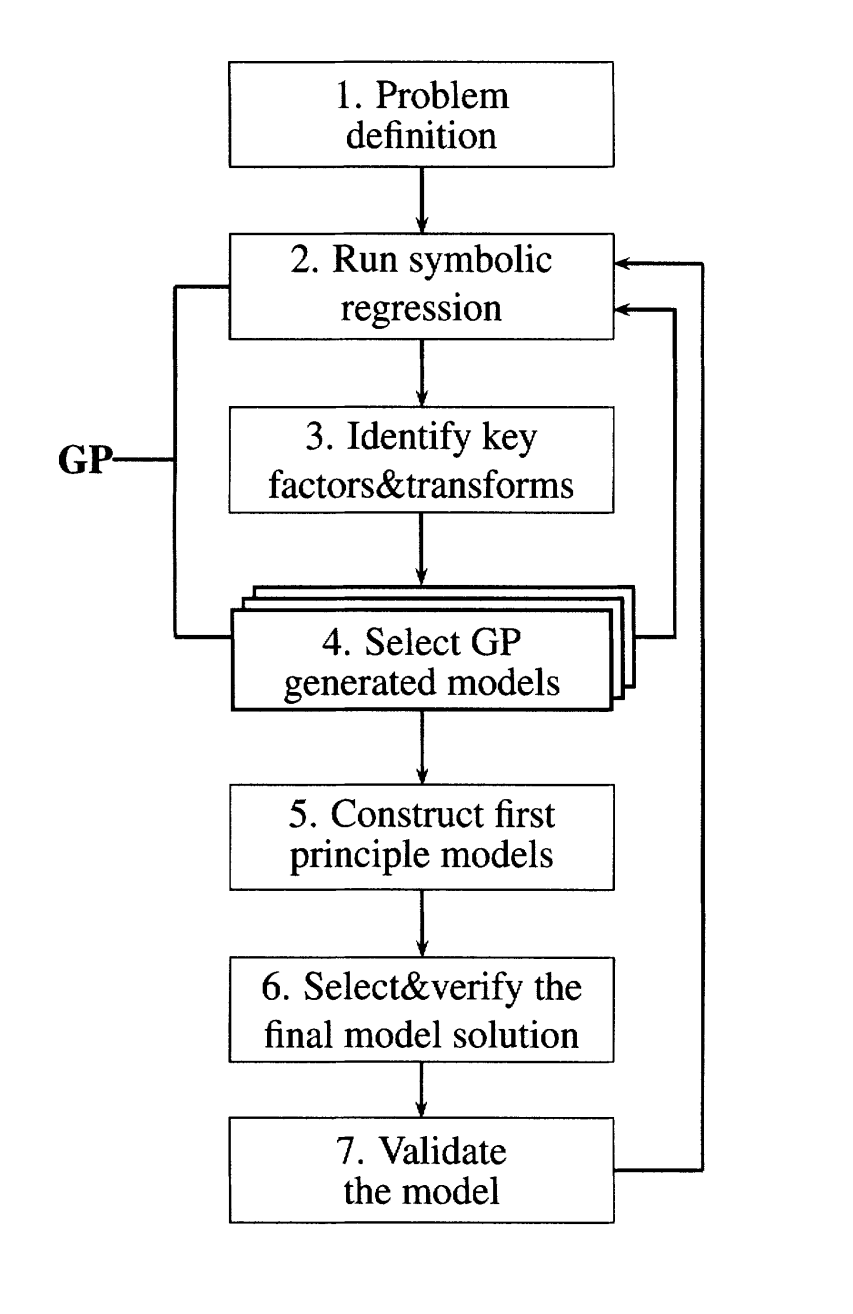
\includegraphics[width=\linewidth,clip]{GP_procedure.png}
	\vspace{-2em}
	\caption{Genetic Programming(GP) iteration procedure: The tree-based GP iteration controls the evolved SR generation and destruct the unpromising offspring.}
	\label{fig:GP_procedure.png}
\end{figure}

A genetic programming typically includes:

\begin{itemize}
	\item{a genetic representation of candidates;}
	\item{a way to create an initial population of candidates;}
	\item{a function measuring the fitness of each candidate;}
	\item{a generation step in which some candidates ``die'', some survive and others reproduce by breeding;}
	\item{a mechanism that recombines genes from breeding pairs and mutates others.}
\end{itemize}



Symbolic regression (SR) is a method to search for a set of mathematical operators that identify an analytical description for the relationships among input and output attributes of the given data set. SR is an NP-hard problem that can be solved using genetic algorithm. Moreover, a standard algorithm used for SR is GP, which specializes for evolving generation and tree structures, e.g, searching for a space of mathematical expressions and minimizing various error metrics. Both the parameters and the form of the equation are subject to search. In SR, many initially random symbolic equations compete via optimization to model experimental data in a most non-traditional manner. New equations are formed by reorganizing and combining previous equations and probabilistically varying their sub-expressions. The algorithm leads to equations that model the experimental data and at the same time reject unpromising solutions.  After an equation reaches a desired level of accuracy, the algorithm terminates, returning equations that may correspond to the intrinsic mechanisms of the initial dataset\cite{SchmidtSR}. The overall procedure summarizing the above steps is shown in \autoref{fig:GP_procedure.png}.

In SR, the represented symbolic expressions are the combination of the genes often represented as a binary tree of algebraic operations with numerical constants and symbolic variables as its leaves. Others include acyclic graphs and grammars \cite{Tsoumakas2007}. The fitness of a particular equation is a numerical measure of how well it agrees with the data, such as the correlation of equations or performance measurement of the experimental data.

The operations can be varied among \textit{abs}, \textit{exp} and \textit{log}, or binary operations, \textit{add, sub, multiply}, and \textit{divide}. If prior knowledge of the initial value is known, which is the so-called domain knowledge, the types of operations available can be chosen ahead of time. The terminal values consist of input attributes of function variables and the constant values.

Mutation in a symbolic expression can change an operator in the binary tree, e.g. it can change the \textit{add} functions into \textit{sub}, change the arguments of an operation such as changing $x+c$ to $ x+x$, delete an operation, such as changing $x+x$ to $ x$ or add an operation by changing $x+x$ to $ x+(x+x)$. If the operator is changed from a binary operation to a constant, one of the two sub-tree branches is discarded and those branches can be chosen randomly.

Crossover of a symbolic expression exchanges sub-trees in the binary trees of the initial expressions.  For example, crossing $f(x) = x^2+c$ and $f(x) = x^2 + sin(x) +x$ could produce a sub tree with $f(x) = x^2+sin(x)$, from which the leaf node $c$ was exchanged with the $sin(x)$ term.

\subsection{Fitness Prediction and Constraint Optimization}  
Fitness function and constraint optimization should be performed by treating every constant as the parameter, which are tuned by an automatic differentiation algorithm\cite{richard2010AD}. The constraint optimization can also be treated as a fitting problem and a customized model with high performance is presented by minimizing an objective function $Q(\alpha)$, which is the sum of squared errors between the experimental data $y$ and the prediction of the SR expression $f(x,\alpha)$ (\autoref{eq:optimization_function}).

\begin{equation} \label{eq:optimization_function}
Q(\alpha) = \sum_{i=0}^{m}(y_i-f(x_i,\alpha))^2
\end{equation}


One of the conditions for SR to work is that differentiable functions such as logistic functions must be incorporated in the SR parsing tree, which encodes formula expression using the combination of the identified markers. Otherwise optimization solutions with one or multiple sets cannot be achieved by the gradient calculation. The gradient of this SR model can generate a continuous search direction, whose information can be used for accelerating this entire process.

The constraint optimization is an iterative procedure which gradually improves the SR model quality using the gradient calculation, starting from initial parameters. As a start, the Jacobian matrix has been calculated from which all numerical values of all initial observed data are derived. The Jacobian matrix is then used to update the parameter vector for the iteration procedure to continue until a specified stopping criterion is reached.

For the calculation of all partial derivatives for the parameter vector $\alpha$, automatic differentiation has been used. In terms of modeling performance and accuracy, automatic differentiation becomes especially competent for constraint optimization. Therefore, all constant values have to be extracted and replaced by an appropriate parameter $\alpha_i$ given in \autoref{eq:function_derivative},

\begin{equation} \label{eq:function_derivative}
\nabla f = \left( \frac{\partial f}{\partial \alpha_1},
\frac{\partial f}{\partial \alpha_2}...
\frac{\partial f}{\partial \alpha_i}\right)
\end{equation}



\begin{figure}[tb]
	\centering
	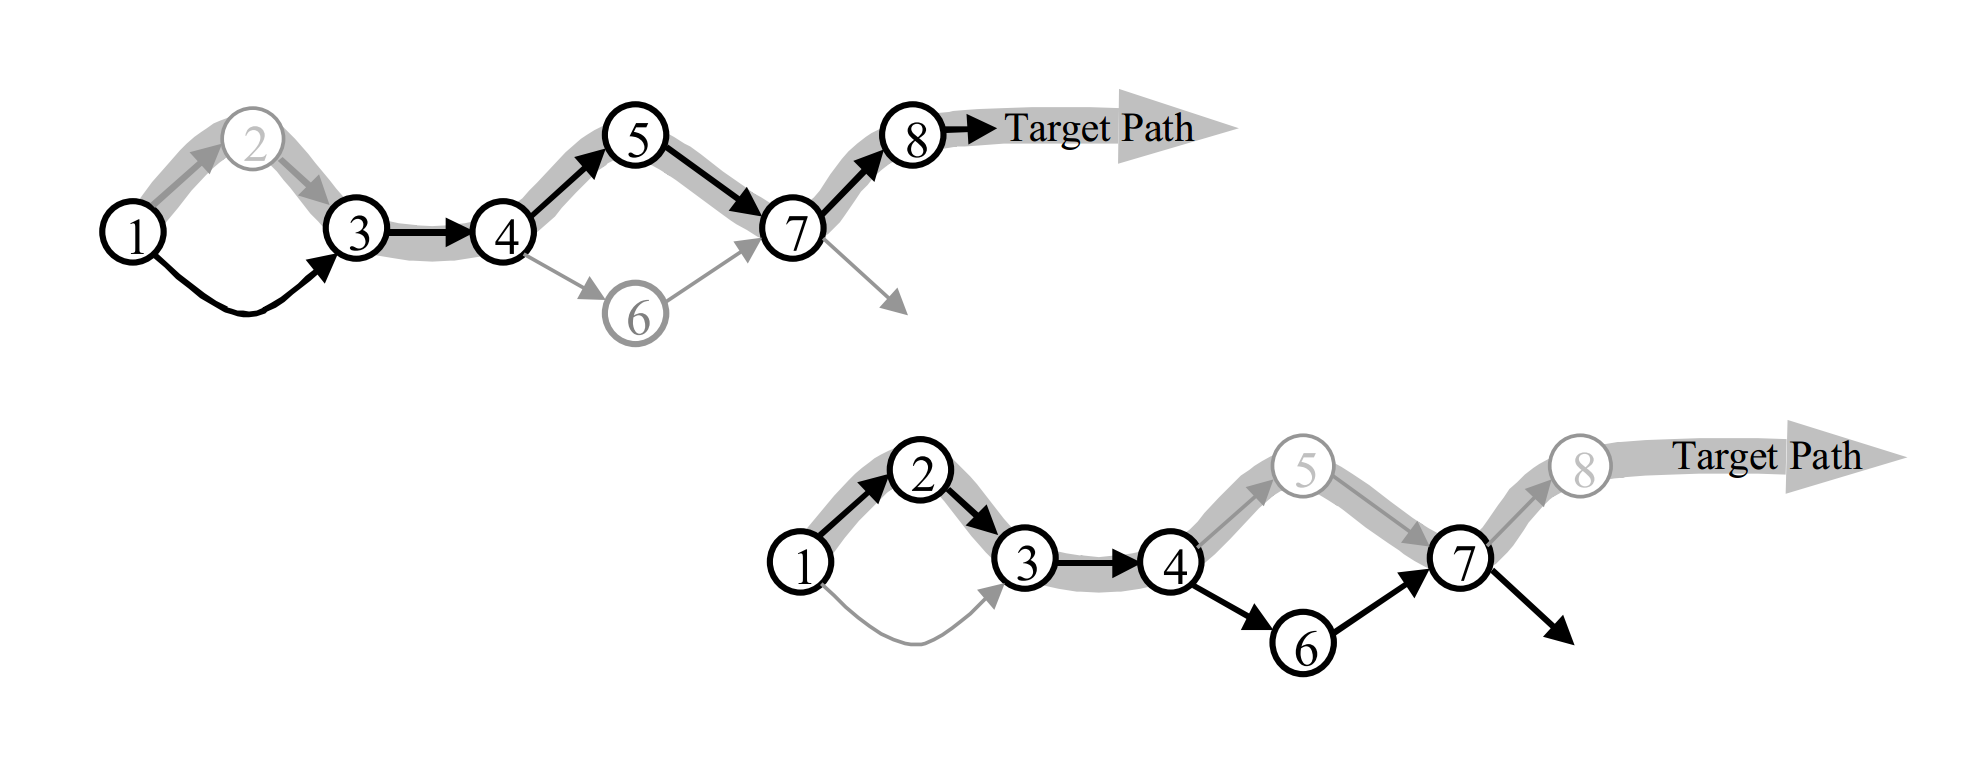
\includegraphics[width=\linewidth,clip]{learning_path.png}
	\vspace{-2em}
	\caption{The
		execution of the first individual (covering the six nodes 1,
		3, 4, 5, 7, and 8 on the target path) will lead to a high
		approximation level if all identical path sections are
		considered for the fitness evaluation. If only the first
		matching path section is measured, the second individual
		(covering five nodes 1, 2, 3, 4, and 7) will lead to a higher
		approximation level than the first one\cite{baresel2002fitness}}.
	\label{fig:learning_path.png}
\end{figure}

\begin{figure*}
	\begin{center}
	\captionsetup{labelformat=empty}
	\caption{Table 1. Comparison of SR with three other modeling techniques (Linear Regression, Neural Networks and Random Forests) which belong to three distinct culture in modeling prediction family\cite{VladislavlevaSR}}.
	
	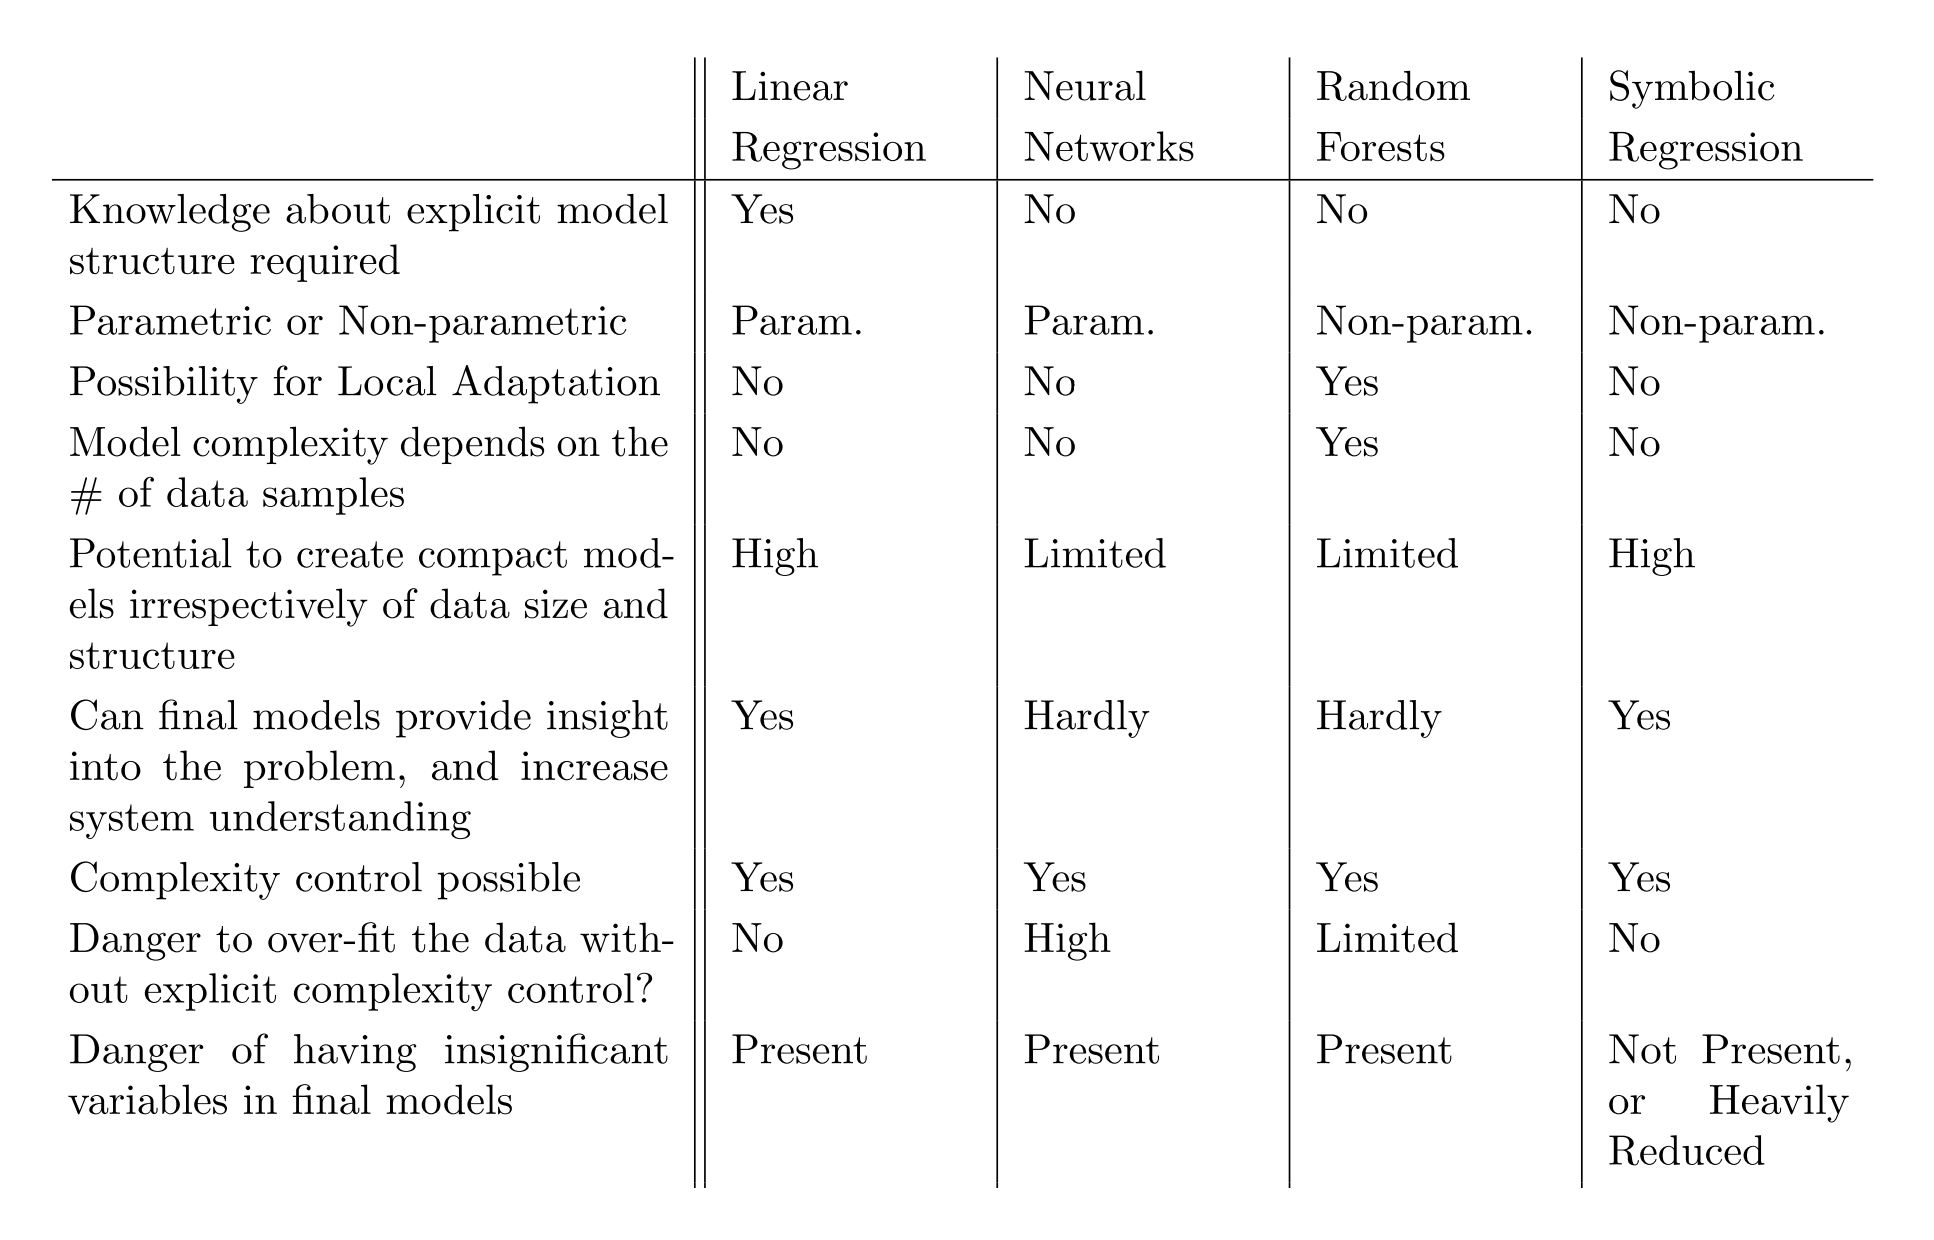
\includegraphics[width=\linewidth]{SR_comparison.png}\end{center}



	\label{Table:SR_comparison}
\end{figure*}



In addition, artificial nodes are introduced in the SR model regarding nonlinear scaling terms. In one iteration, the start values for the SR model are the previously extracted constraint values in terms of additive and multiplicative scaling terms. The length of all path sections has been used as an approximation. Because a high fitness value can be achieved by covering the desired path to the convergence criterion from the target initial start, the combination of two such nodes may lead to considerably better offspring. This is shown in \autoref{fig:learning_path.png}. The algorithm is stopped after a customized number of iterations. The quality of individual parameters for optimized constants would be updated. Meanwhile, the optimization starts from the same values which are automatically retrieved in the model. This procedure is repeated many times by tuning the parameter vectors from which the individuals with a boolean value are flagged. 


The designed algorithm describing necessary steps for optimizing the constraint of the proposed SR model is given as Algorithm \autoref{algo:deepnmfalgo}. In the literature, the SR method has been utilized in many application areas. SR is able to understand the data and build a descriptive model derived. Most importantly it provides certain insights about the data and the model. Table 1 provides comparison among several methods including SR. In section 3, we demonstrate the application of SR to the analysis of oil sands ore properties. 


\begin{algorithm}[!htb]
	\caption{This proposed algorithm for training a SR model: Initially we approximate the factors greedily using the automatic differentiation algorithm \cite{ding2010convex} and then fine-tune the factors until the convergence criterion is satisfied.}
	
	\begin{algorithmic}
		\label{algo:deepnmfalgo}
		\STATE {\bfseries Input:} {${\bs X} \in \mathbb{R}^{p\times n}$, a list of initial constraint values }
		\STATE {\bfseries Output:} {weight matrices ${\bs Y}_i$}
		\STATE {}
		\STATE {Add scaling tree nodes}
		\STATE {Transform the tree for constraint optimization}
		\WHILE{Stopping criterion not reached}
		\STATE	{Calculate the gradient with automatic differentiation}
		\ENDWHILE
		
		\STATE{Calculate quality with optimized constraint}
		
		
		\REPEAT
		\IF{Update Constraint}
		\STATE{Retrieve optimized constraint}
		\ENDIF
		\UNTIL{Stopping criterion is reached}
		
	\end{algorithmic}
\end{algorithm}


\section{Implementation Procedure}\label{sec:experiments}




\subsection{Problem Setup}

To implement the SR based genetic programming, we will perform the following procedure:
     	\begin{enumerate}
     		\item  Binary representation conversion. 
     		\vskip 0.1in
     		\item  Initial population setup.
     		\vskip 0.1in
     		\item  Fitness measurement.
     		\vskip 0.1in
     		\item  Death, breeding, and mutation.
     	\end{enumerate}
     	
For this study, we chose six decimal digits of accuracy to create the possible solutions, when converting the dataset using binary representation. Six decimal digits of accuracy corresponds to about
		22 binary digits. A 22 digit binary string $b$ can be converted
		to an integer $k$ which is given by:
\begin{equation}
		k = \sum_{i=1}^{22} b_i \cdot 2^{i-1}
\end{equation}
		The integer $k$ is then converted to a real number $u$ between 0 and 1 by:
\begin{equation}	
		u = k / ( 2^{22}-1)
\end{equation}
		and $u$ is again  converted to a real number $r$ between -1 and +2 by:
\begin{equation}	
		W = -1 + 3 \cdot u
\end{equation}
		so now we have a mapping between genetic information $b$ and
		the objective $W$.

\subsection{Implementation Details}

		Each candidate is a string of 22 binary digits, which can be treated as an integer vector.
		\vskip 0.1in
		We choose a population of $n = 50$ candidates, creating a 2 dimensional array of size $50 \times 22$.
		\vskip 0.1in
		A random initial population that can be selected as an array of 0's and 1's is given below as an example.
		
		\begin{verbatim}
		
		
		i  ----------b-----------     ----W----
		#1  1000101110110101000111  =  0.637197
		#2  0000001110000000010000  = -0.958973
		...
		#50 1110000000111111000101  =  1.627888
		\end{verbatim}
The best candidate $W$ is to search the optimized quantity $R(T)$.
				\vskip 0.1in
		In this study, the initial fitness function is chosen as follows:
\begin{equation}	
				R(T) = T \sin ( 10 \pi T ) + 1
\end{equation}
		
		Second, the iteration begins by measuring the fitness of each candidate as given below:
		\begin{verbatim}
		i  -----------b----------       --R(T)--
		
		#1  1000101110110101000111   => 1.586345
		#2  0000001110000000010000   => 0.078878
		...
		#50 1110000000111111000101   => 2.250650
		\end{verbatim}	

		Based on the fitness results, the following steps are performed for the next
		generation:
		\begin{itemize}
			\item {Out of the 50 candidates, remove 10 candidates with the lowest fitness; }
			\item {Let the 10 candidates with the highest fitness breed in pairs, creating 10 new candidates;}
			\item {Randomly select 2 of the nonbreeding, nondying candidates for mutation;}
		\end{itemize}
		\vskip 0.1in
		The size of the new population remains unchanged when it contains the best candidates from the previous population. The 10 candidates with lower score are replaced by new offspring of higher fitness score. For the intermediate 30 candidates, we modify two candidates randomly by mutation and keep 28 candidates unchanged.
		\vskip 0.1in
		For mutation, a candidate $i$ can be picked to mutate. It is known that each candidate
		has 22 bits of genetic information. For example, one can pick index $j$ between 1 and 22 and
		flip that bit:

		\begin{verbatim}
		b(i,j) = 1 - b(i,j)
		\end{verbatim}
		\vskip 0.1in
		For breeding, we assume parents $i_1$ and $i_2$ creating children $i_3$ and $i_4$.
		To achieve this, an index $j$ between 1 and 21 is chosen and parental information can then be spliced together as follows:
		\begin{verbatim}
		b(i3,1:j) = b(i1,1:j)& b(i3,j+1:22)
		b(i4,1:j) = b(i2,1:j)& b(i4,j+1:22)
		\end{verbatim}

		Given the candidate \#50 which is:
		\begin{verbatim}
		i  -----------b----------     --R(T)--
		
		#50 1110000000111111000101 => 2.250650
		\end{verbatim}
		If the fifth gene in this candidate is mutated, then the result is
		\begin{verbatim}
			1110100000111111000101  =>  -0.082257
		\end{verbatim}
		but if the 10th gene is mutated, then the following result is obtained:
		\begin{verbatim}
			1110000001111111000101  =>  2.343555
		\end{verbatim}
		Thus, a mutation process can be controlled to improve the fitness value.
		
The following shows the results of breeding. For example, we make candidates \#2 and \#50 breed, 
		\begin{verbatim}
		i  -----------b----------        --R(T)--
		#2  0000001110000000010000   =>  0.078878
		#50 1110000000111111000101   =>  2.250650
		\end{verbatim}
		The crossover point is defined as a selection of parental information to generate offspring. 
		If the crossover point is after $j=5$, the two children will be as follows. 
		\begin{verbatim}
		-----------b----------      --R(T)--
		0000000000111111000101  =>  0.940865
		1110001110000000010000  =>  2.459245
		\end{verbatim}
		It is obvious that one child has a significant increase in the fitness function.

The GP procedure is terminated after 441 iterations. For the simulated data, intermediate results from the symbolic regression algorithm in several steps are shown in Table 2. The final results and the performance validation are included in Section 4. 

\begin{table}[hptb]\label{tab:iteration}
		\begin{center}
			\captionsetup{labelformat=empty}
			
			\caption{Table 2. Results of fitness function generation, for a variable number of combinations of input attributes from the simulation data.}
			
			\begin{tabular}{|r|l|}
				\hline
				Gen & $\hat{R}(T)$ \\
				\hline
				1 & $T \sin ( 10 \pi T ) + 1$ \\
				6 & $T$ \\
				8 & $16.2+T$ \\
				9 & $34.3+1.08T$ \\
				10 & $61.7+29\sin(4.14+0.0519T)$ \\
				12 & $61.7+43.9\sin(4.23+0.0517T)$ \\
				39 & $18.3+73logistic(0.465T-16.6)$ \\
				40 & ... \\
				51 & ... \\
				99 & $18.2+0.000165T^2 +72.3logistic(0.468T-16.7)$ \\
				441 & ... \\
				\hline
			\end{tabular}

		\end{center}
\end{table}

\section{SR descriptor results} \label{sec:related}

The oil sands data set contains three inputs variables: Temperature (T), pH, and Clay fines (Cf). The output is oil sands processability recovery rate (R). Due to lack of industrial data, we use data from laboratory experiments together with the generated simulation data. The simulation data set contains 1000 data points, which are generated based on known and empirical knowledge about relations among variables. Furthermore, it is noted that symbolic regression requires repeated simulation from multiple data generation. This can be achieved by adding noises and changing noise profiles to repeat the simulation.

Applying the SR to the simulated oil sands dataset and after 441 iterations,  led to a descriptor (i.e. a mathematical expression) for the factor analysis of oil sands recovery rate. 
In this section, we will construct and evaluate how well the fitness function is performed by calculating the root mean square error for the difference between the original data and the reconstruction by the descriptor for all input factors. Note that, in order to have comparable results, all of the fitness functions have the same termination criterion rules. We have set the maximum amount of iterations to 1000 (usually ${\sim}100$
iterations are enough). As explained in Section 3, the final descriptor obtained by the SR is shown as \autoref{eq:deep_nmf_linear_cost}, which presents several sensible markers and their relationships constructed from the data used in this study. 

The SR descriptor shows that the SR method renders a clear reconstruction for the simulation data than the other methods, in which an analytical expression is obtained. This descriptor, to a certain degree, demonstrates sensible features of several input attributes. Such an descriptor can also be improved by integrating physical insights as constraints, such as function candidate blockers or generators during SR iterations. 


\begin{align} \label{eq:deep_nmf_linear_cost}
\notag  \bs R &= 0.39\cdot T \cdot pH + 25.5\cdot logistic(0.0597 \cdot pH)\\\notag 
&\qquad + 0.00783 \cdot pH^2 \cdot Cf^{-3} + 5.79 \cdot logistic(0.001 \cdot pH^3)\\\notag 
&\qquad +0.049 \cdot T^2 -0.035 \cdot T^3-0.002\cdot T \cdot pH \cdot Cf^{-2}\\\notag 
&\qquad + 0.00369 \cdot Cf^{-4} \cdot logistic(0.001 \cdot Cf^{-3})\\\notag
&\qquad +...\\
\end{align}

It is noted that the terms shown in Equation 7 are considered to be the key factors, and ... represents the other terms of lower importance. 

Figure 4 shows the descriptor curve in comparison with the training data ($\circ$) which are real laboratory data and a few selected simulation data. As one would expect, the few number of laboratory data alone do not contain enough information to detect recovery rate.
However, with the simulation data, the SR descriptor
has the possibility of reviving the trend of recovery rate as a function of temperature. The results in Figure 4 clearly show an excellent description of recovery dependence on temperature in Equation 7.


  \begin{figure}[tb]
  	\centering
  	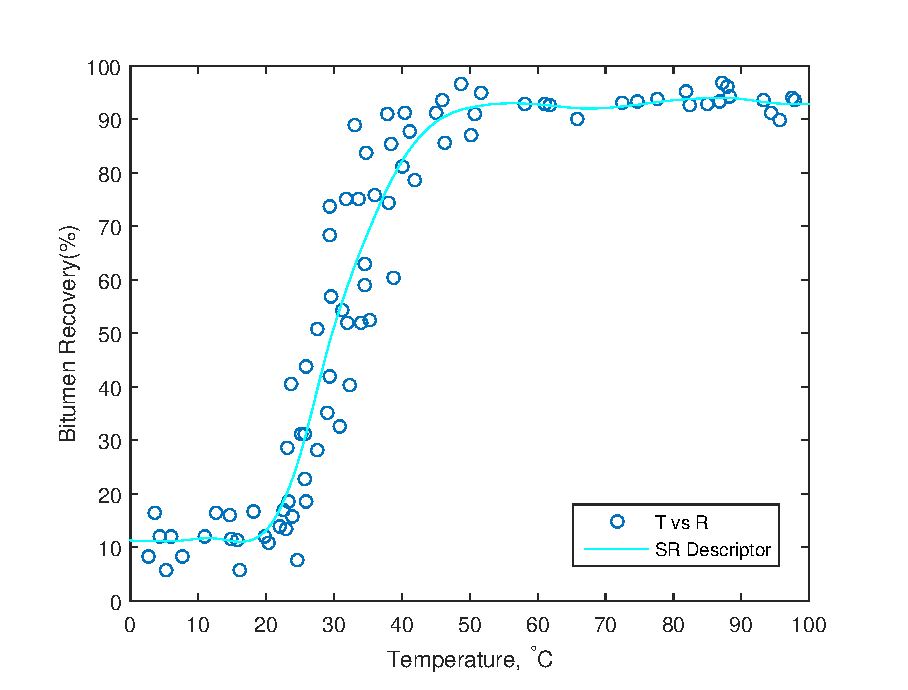
\includegraphics[width=\linewidth,clip]{T_SR.eps}
  	\vspace{-2em}
  	\caption{Symbolic regression prediction of the relationship between recovery and temperature.}
  	\label{fig:T_SR}
  \end{figure}
  
  


  
  \begin{figure}[tb]
  	\centering
  	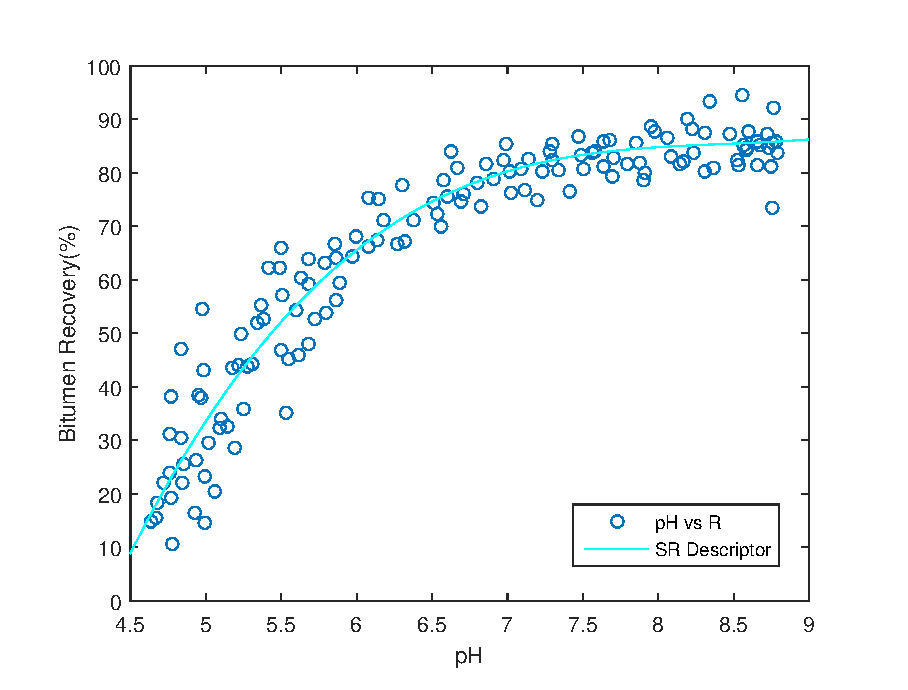
\includegraphics[width=\linewidth,clip]{pH_SR.eps}
  	\vspace{-2em}
  	\caption{Symbolic regression prediction of the relationship between recovery and pH.}
  	\label{fig:pH_SR}
  \end{figure}
  
  
  \begin{figure}[tb]
  	\centering
  	\includegraphics[width=\linewidth,clip]{Cf_SR.eps}
  	\vspace{-2em}
  	\caption{Symbolic regression prediction of the relationship between recovery and Cf.}
  	\label{fig:CF_SR}
  \end{figure}


Figure 5 shows clearly how the bitumen recovery varies with slurry pH: starting from 10\%  at pH 4.5 with a rapid increase with increasing pH to 7 followed by a slow increase to reach around the 85\%  at pH 9.0. The results in Figure 6  show an opposite trend of decreasing recovery rate with increasing clays content.

Note that the shape of the curve strongly depends on the
fitness function $Q(\alpha)$ in Equation 1. General speaking, more information from data points should not lead to a decrease in predictability.
Thus, the SR descriptor from the simulation data set has richer interpolation in features domain. Counterintuitively, the descriptor from the mixed dataset becomes more reliable by changing parameter $\alpha_i$ in Equation 2. Despite that, we can use $\alpha_i$ to influence the shape of the SR curve. The most accurate model of the mixed data
set is still the most accurate model overall.


To assess the quality and accuracy of the descriptor, comparison of the predicted results from the descriptor and the original laboratory data is performed, and the comparison results are shown in Figures 7-9. \autoref{fig:t_comparison.png} shows the constructed relationship of the recovery rate versus the temperature, compared to the original experiment data used. By increasing the clay fines from 20 wt\% to 30 wt\%, two curves are generated by SR descriptor and yet still share the same trending with respect to the bitumen recovery affected by temperature from 0 to 100 degree.

Two other input attributes, such as pH value and the clay fines, and how they affect the recovery are also evaluated. \autoref{fig:ph_comparison.png} and \autoref{fig:Cf_comparison.png} show the comparison in prediction accuracy when changing temperature on the feature representations. From these figures, it is shown that the SR descriptor presents meaningful interpretation and more clear understanding of the data.



  \begin{figure}[tb]
       \centering
       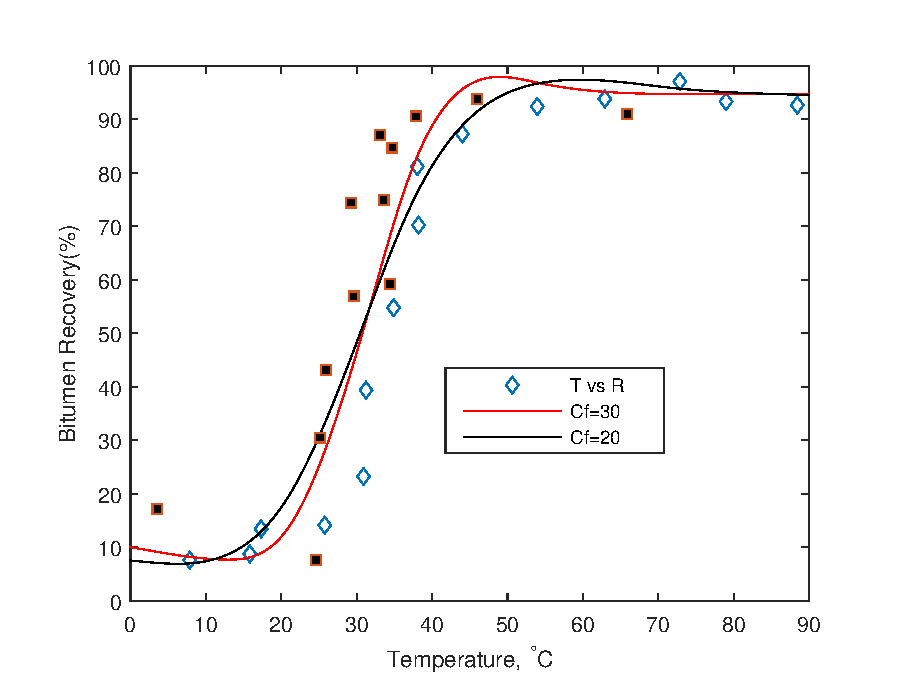
\includegraphics[width=\linewidth,clip]{T_comparison.eps}
       \vspace{-2em}
                \caption{Symbolic regression prediction of the relationship between recovery and temperature. Blue hollow square indicate actual data points. By altering clay fines amount to 30\%, red solid curve is visualized compared with original dark solid curve.}
       \label{fig:t_comparison.png}
  \end{figure}
    \begin{figure}[tb]
         \centering
         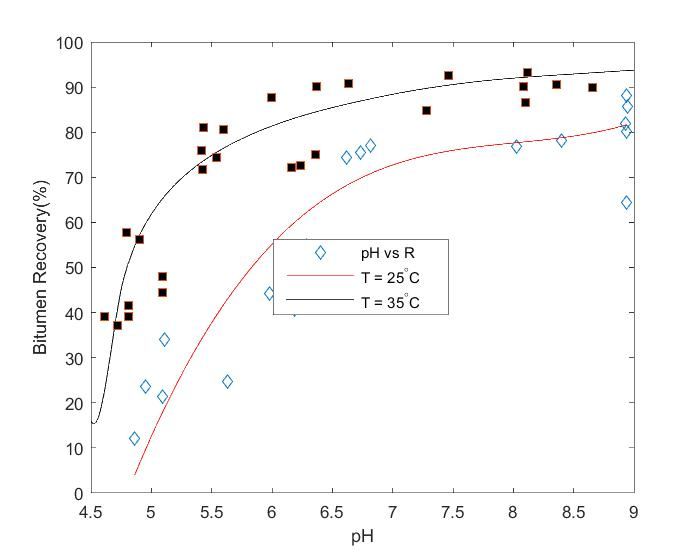
\includegraphics[width=\linewidth,clip]{ph_comparison.eps}
         \vspace{-2em}
                  \caption{Symbolic regression prediction of the relationship between recovery and pH. Blue hollow square indicate actual data points. The difference between red and dark visualized curves is 10 degree alteration of temperature.}
         \label{fig:ph_comparison.png}
    \end{figure}
    
        \begin{figure}[tb]
        	\centering
        	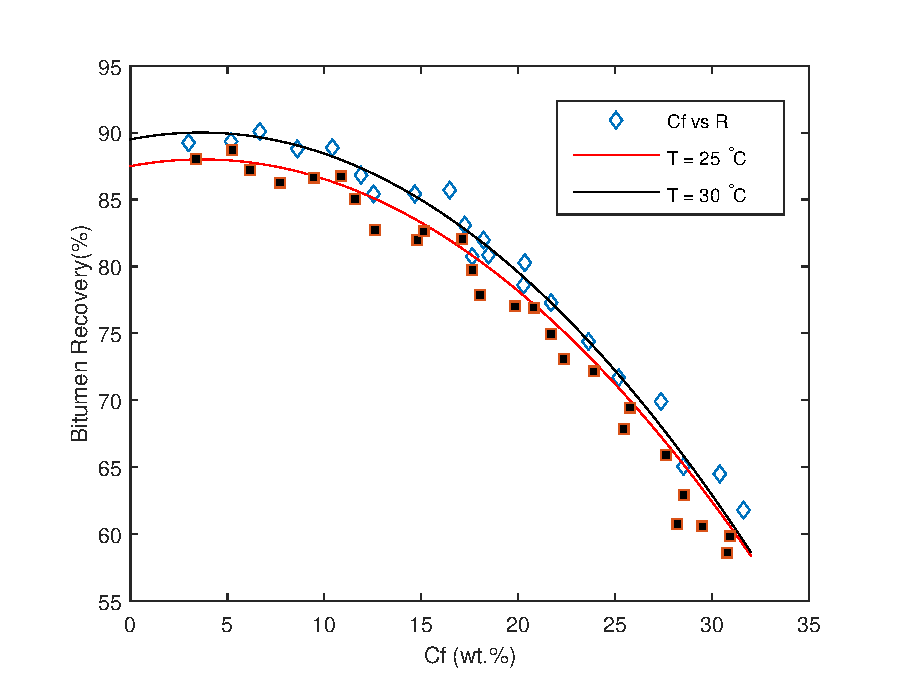
\includegraphics[width=\linewidth,clip]{Cf_comparison.eps}
        	\vspace{-2em}
        	\caption{Symbolic regression prediction of the relationship between recovery and clay fines. Blue hollow square indicate actual data points. The difference between red and dark visualized curves is 5 degree alteration of temperature. }
        	\label{fig:Cf_comparison.png}
        \end{figure}
  
  
  In Figure 10, the RMS errors between the SR result and the two original datasets,  which are the training dataset and the test dataset, are compared respectively.
  The RMS scores are 0.24534 and 0.2443, respectively. 
  
       \begin{figure}[tb]
       	\centering
       	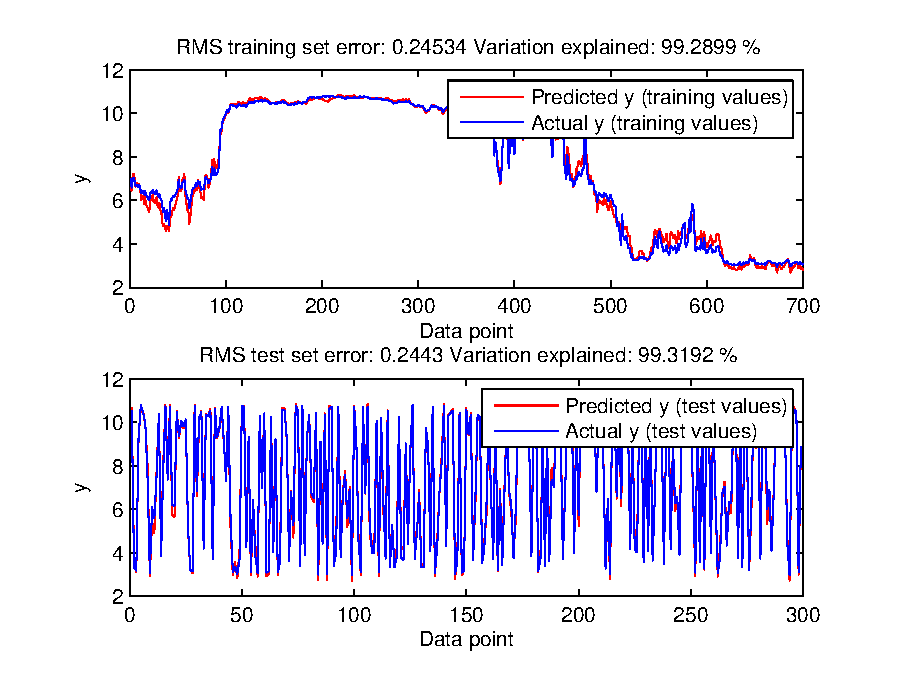
\includegraphics[width=\linewidth,clip]{sensitivity.eps}
       	\vspace{-2em}
       	\caption{Symbolic regression model performance.}
       	\label{fig:sensitivity.eps}
       \end{figure}
       	

Finally, we evaluate the residuals between the observed value of the dependent variable and the predicted value (\autoref{fig:sensitivity2.eps}). Both the training and testing data indicate a non random patterns and show a good fit for the SR model.





         \begin{figure}[tb]
                \centering
                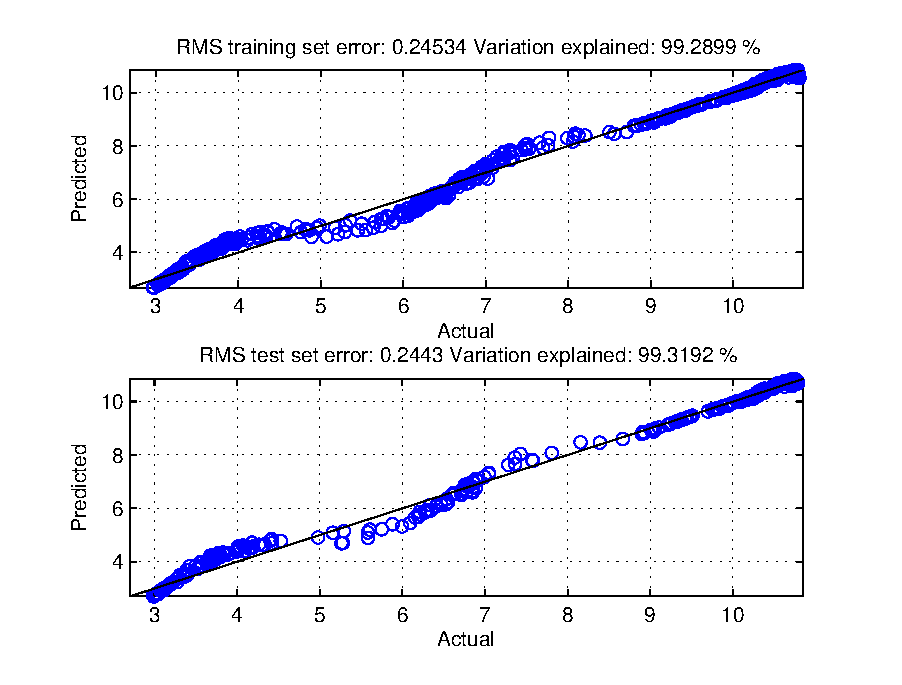
\includegraphics[width=\linewidth,clip]{sensitivity2.eps}
                \vspace{-2em}
                         \caption{Symbolic regression prediction performance.}
                \label{fig:sensitivity2.eps}
           \end{figure}


\section{Conclusion} % (fold)
\label{sec:conclusion}
We have introduced a novel symbolic regression model for oil sands recovery prediction, fitness function blockers, which are able to select an optimum combination of function candidates and a set of mathematical operators so that the data can be described by the constructed mathematical descriptor. Furthermore, we show that the proposed technique is able to understand a combination of representations for oil sands recovery with respect to the sensible markers obtained using a simulation oil sands data.

One important future work is to experiment with real world recovery datasets, especially the industrial plant data.

% use section* for acknowledgement
%\ifCLASSOPTIONcompsoc
  % The Computer Society usually uses the plural form
%  \section*{Acknowledgments}
%\else
  % regular IEEE prefers the singular form
%  \section*{Acknowledgment}
%\fi


% Can use something like this to put references on a page
% by themselves when using endfloat and the captionsoff option.
\ifCLASSOPTIONcaptionsoff
  \newpage
\fi\bibliographystyle{IEEEtran}

\begin{thebibliography}{10}
	\providecommand{\url}[1]{#1}
	\csname url@samestyle\endcsname
	\providecommand{\newblock}{\relax}
	\providecommand{\bibinfo}[2]{#2}
	\providecommand{\BIBentrySTDinterwordspacing}{\spaceskip=0pt\relax}
	\providecommand{\BIBentryALTinterwordstretchfactor}{4}
	\providecommand{\BIBentryALTinterwordspacing}{\spaceskip=\fontdimen2\font plus
		\BIBentryALTinterwordstretchfactor\fontdimen3\font minus
		\fontdimen4\font\relax}
	\providecommand{\BIBforeignlanguage}[2]{{%
			\expandafter\ifx\csname l@#1\endcsname\relax
			\typeout{** WARNING: IEEEtran.bst: No hyphenation pattern has been}%
			\typeout{** loaded for the language `#1'. Using the pattern for}%
			\typeout{** the default language instead.}%
			\else
			\language=\csname l@#1\endcsname
			\fi
			#2}}
	\providecommand{\BIBdecl}{\relax}
	\BIBdecl
	
	
	\bibitem{Masliyah2004}
	Masliyah, J, et al. "Understanding water‐based bitumen extraction from Athabasca oil sands." The Canadian Journal of Chemical Engineering 82.4 (2004): 628-654.
	
	\bibitem{Fong2004}
	N. Fong, S. Ng and K. Chung. "A Two Level Fractional Factorial Design to Test the Effect of Oil Sands Composition and Process Water Chemistry on Bitumen Recovery from Model Systems". The Canadian Journal of Chemical Engineering. Volume 82, Issue 4, 782-793,2004
	
	\bibitem{ZhangANN}
	Q. Zhang, R. Sawatzky, E. Wallace, M. London, and S. Stanley,
	"Artificial neural network modelling of oil sands extraction processes"
	Journal of Environmental Engineering and Science, 2003.
		

			
	\bibitem{MichalewiczGP}
	Z. Michalewicz,
	"Genetic Programming + Data Structures = Evolution Programs"
	Third Edition, Springer, 1996.
	
	\bibitem{brunet2004metagenes}
	J.-P. Brunet, P.~Tamayo, T.~R. Golub, and J.~P. Mesirov, ``Metagenes and
	molecular pattern discovery using matrix factorization,'' \emph{PNAS}, vol.
	101, no.~12, pp. 4164--4169, 2004.
	
	\bibitem{devarajan2008nonnegative}
	K,~Devarajan, ``Nonnegative matrix factorization: an analytical and
	interpretive tool in computational biology,'' \emph{PLoS computational
	biology}, vol.~4, no.~7, p. e1000029, 2008.
	
	\bibitem{KozaGP}
Koza,R. "Genetic programming II: Automatic discovery of reusable subprograms." Cambridge, MA, USA (1994).

	\bibitem{berry2005email}
	M.~W. Berry and M.~Browne, ``Email surveillance using non-negative matrix
	factorization,'' \emph{Computational \& Mathematical Organization Theory},
	vol.~11, no.~3, pp. 249--264, 2005.
	
	\bibitem{BurkardtImageGA}
Freitas, Alex A. "A genetic programming framework for two data mining tasks: classification and generalized rule induction." Genetic programming (1997): 96-101.
	
	\bibitem{zafeiriou2006exploiting}
	S.~Zafeiriou, A.~Tefas, I.~Buciu, and I.~Pitas, ``Exploiting discriminant
	information in nonnegative matrix factorization with application to frontal
	face verification,'' \emph{TNN}, vol.~17, no.~3, pp. 683--695, 2006.
	
	\bibitem{kotsia2007novel}
	I.~Kotsia, S.~Zafeiriou, and I.~Pitas, ``A novel discriminant non-negative
	matrix factorization algorithm with applications to facial image
	characterization problems.'' \emph{TIFS}, vol.~2, no. 3-2, pp. 588--595,
	2007.


	\bibitem{weninger2012optimization}
	F.~Weninger and B.~Schuller, ``{Optimization and parallelization of monaural
		source separation algorithms in the openBliSSART toolkit},'' \emph{Journal of
		Signal Processing Systems}, vol.~69, no.~3, pp. 267--277, 2012.
	
		
	\bibitem{HouckGA}
	C. Houck, J. Joines, and M. Kay,
	"A Genetic Algorithm for Function Optimization: A Matlab Implementation"
	NCSU-IE Technical Report 95-09, 1996.
	

	
	\bibitem{ding2010convex}
	C.~H. Ding, T.~Li, and M.~I. Jordan, ``Convex and semi-nonnegative matrix
	factorizations,'' \emph{IEEE TPAMI}, vol.~32, no.~1, pp. 45--55, 2010.
	
	\bibitem{SchmidtSR}
	M. Schmidt, H. Lipson, "Distilling Free-Form Natural Laws from Experimental Data",  Science, 324: 81-85, pp.2009
	
	\bibitem{Tsoumakas2007}
	G.~Tsoumakas and I.~Katakis, ``{Multi-label classification: An overview},''
	\emph{International Journal of Data Warehousing and Mining}, vol.~3, pp.
	1--13, 2007.
	
	\bibitem{Herrero2001}
	J.~Herrero, A.~Valencia, and J.~Dopazo, ``{A hierarchical unsupervised growing
		neural network for clustering gene expression patterns.}''
	\emph{Bioinformatics (Oxford, England)}, vol.~17, pp. 126--136, 2001.
	
	\bibitem{VladislavlevaSR}
	E,~Vladislavleva,"{Model-based problem solving through symbolic regression via pareto genetic programming.}"
	\emph{PhD thesis, (Tilburg University,Tilburg)}, the Netherlands,2008.


	\bibitem{baresel2002fitness}
			André Baresel, Harmen Sthamer, and Michael Schmidt, “{Fitness Function Design To Improve Evolutionary Structural Testing},” \emph{Proceedings of the Genetic and Evolutionary Computation Conference}, 1329-1336,2002.

	

    \bibitem{richard2010AD}
	Neidinger, D. "{Introduction to Automatic Differentiation and MATLAB Object-Oriented Programming.}" \emph{SIAM Review 52 (3): 545–563},2010.

	

	
	
	
\end{thebibliography}



% trigger a \newpage just before the given reference
% number - used to balance the columns on the last page
% adjust value as needed - may need to be readjusted if
% the document is modified later
%\IEEEtriggeratref{8}
% The "triggered" command can be changed if desired:
%\IEEEtriggercmd{\enlargethispage{-5in}}

% references section





\vfill

% that's all folks
\end{document}


